% !TeX spellcheck = en_US
\documentclass[]{article}

\usepackage[utf8]{inputenc}

\usepackage{natbib}
\usepackage{graphicx}

\usepackage[english]{babel}
\usepackage{amsmath}
\usepackage{amsfonts}
\usepackage{amssymb}

\usepackage[T1]{fontenc}
\usepackage{listingsutf8}
\lstset{literate={č}{{\v c}}1 {š}{{\v s}}1 {ž}{{\v z}}1}
\lstset{basicstyle=\ttfamily, language=matlab}


\title{Homework 2}
\author{Lovro Habjan}

\begin{document}

\maketitle

\section{Introduction}

For homework 2 we implemented two ways of computing \textit{B\'ezier curves} -
directly and with the De Casteljans algorithm. We are given a set of control
points $b_i, i = 0, 1, 2, ..., n$ in the plane $\mathbb{R}^2$.

\section{Methods}

\subsection{Direct algorithm}

With $b_i$, $i = 0, 1, 2, ..., n$, the method to directly compute the B\'ezier
algorithm is:
\begin{equation*} \textbf{b}(t) = \sum_{i = 0}^{n} b_i B^n_i (t), B^n_i(t) =
\binom{n}{i} t^i (1-t)^{n-i}, t \in [0, 1]
\end{equation*}

We implemented the algorithm in MATLAB. The input parameter $\textbf{b}$ is a
matrix of size $2 \times (n + 1)$, where each line represents a control
point. We modify the direct algorithm so the indexes are used correctly. The
result is a vector $v \in \mathbb{R}^2$. The code for the algorithm is:
\begin{lstlisting}
function v = computeDirectly(b, t)
    v = [0, 0];
    [nPlusOne, ~] = size(b);
    for i = 1:nPlusOne
        v = v + binomialGamma(nPlusOne-1, i-1) * t^(i-1) * ...
            (1-t)^(nPlusOne-i) * b(i,:);
    end
end
\end{lstlisting}

Where we computer the binomial as:
\begin{equation*}
	\binom{n}{k} = \frac{\Gamma(n+1)}{\Gamma(k+1) \Gamma(n-k+1)}
\end{equation*}

\subsection{De Casteljans algorithm}

De Casteljans algorithm is defined recursively:
\begin{align*} \textbf{b}^0_i(t_0) &= b_i \\ \textbf{b}^r_i(t_0) &= (1 - t_0)
\textbf{b}^{r-1}_i(t_0) + t_0 \textbf{b}^{r-1}_{i+1}
\end{align*}

The naive implementation of this algorithm is of exponential complexity, as we
compute the same $\textbf{b}_i^r$ multiple times. We can achieve a better time
complexity, as we observe that to compute $\textbf{b}_r^i$ we only need
$\textbf{b}_{r-1}^i$ for all $i = 0, 1, ..., n - r$. Because
$\textbf{b}_i^0 = b_i$, we can start with $r = 0$ and compute $\textbf{b}_i^r$
for every $r = 1, 2, ..., n$. Element $\textbf{b}^r_i$ only needs elements
$\textbf{b}^{r-1}_i$ and $\textbf{b}^{r-1}_{i+1}$, we can modify the matrix
in-place. The final result is stored in $\textbf{b}^n_0$. The code in MATLAB for
the algorithm, where indexes are adjusted:

\begin{lstlisting}
function v = deCastiljas(b, t)
    [nPlusOne, ~] = size(b);
    for i = (nPlusOne-1):-1:1
        for j = 1:i
            b(j,:) = (1-t) * b(j,:) + t * b(j+1,:);
        end
    end
    v = b(1,:);
end
\end{lstlisting}

\section{Results}

We tested the algorithms on 4 different test cases. First two were small,
containing 4 different points. The third test case had 100 randomly selected
control points with larger coordinates and the fifth had 10 control points with
larger coordinates $x, y \in [1000, 10000]$. We measured the difference between
the results of both algorithms for values $t \in [0, 1]$ with 0.01 increment. We
used the following norms:
\begin{itemize}
	\item Euclid norm: $\lvert \lvert x \rvert \rvert_2 = \sqrt{\sum_{i = 1}^{n}
x_i^2}$
	\item Maximum norm: $\lvert \lvert x \rvert \rvert_\infty = \max_{1 \leq i
\leq n} \lvert x_i \rvert$
	\item Taxi norm: $\lvert \lvert x \rvert \rvert_1 = \sum_{i = 1}^{n} \lvert
x_i \rvert$
\end{itemize}

Figure~\ref{fig:01-curve} and~\ref{fig:02-curve} show the small test cases. The
difference between results are shown in~\ref{fig:01-diffs}
and~\ref{fig:02-diffs}. We see that the difference between results is small
(order of $10^{-16}$). Figure~\ref{fig:03-curve} shows the curve for test case
3, with the differences shown in figure~\ref{fig:03-diffs}. We see that the
order of difference is $10^{-13}$. This shows that algorithms lose accuracy with
larger numbers. The curve for test case 4 is shown in
figure~\ref{fig:04-curve}. The differences are shown in
figure~\ref{fig:04-diffs}. We see the biggest order of difference ($10^{-11}$)
for test case 4, where we used larger numbers than in previous test cases.

\begin{figure}
  \centering
  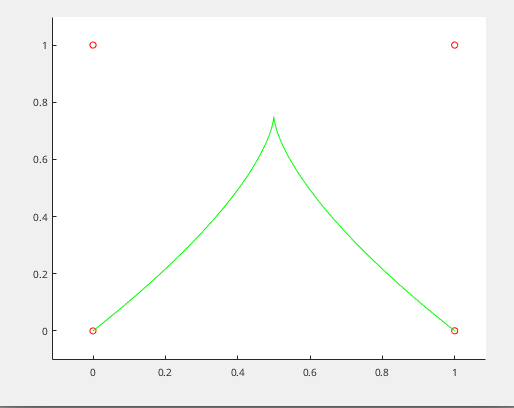
\includegraphics[width=0.8\linewidth]{figs/01-curve.png}
  \caption{Curve for test 1}
  \label{fig:01-curve}
\end{figure}

\begin{figure}
  \centering
  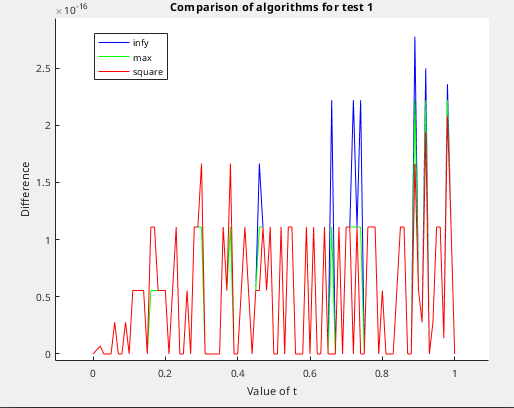
\includegraphics[width=0.8\linewidth]{figs/01-diffs.png}
  \caption{Comparison of algorithms for test 1}
  \label{fig:01-diffs}
\end{figure}

\begin{figure}
  \centering
  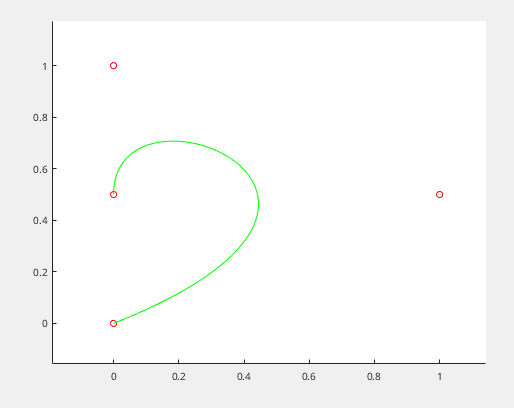
\includegraphics[width=0.8\linewidth]{figs/02-curve.png}
  \caption{Curve for test 2}
  \label{fig:02-curve}
\end{figure}

\begin{figure}
  \centering
  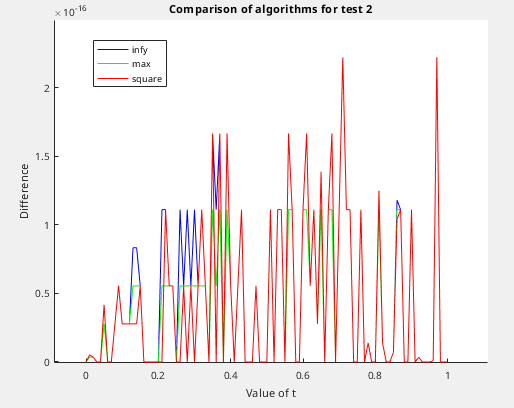
\includegraphics[width=0.8\linewidth]{figs/02-diffs.png}
  \caption{Comparison of algorithms for test 2}
  \label{fig:02-diffs}
\end{figure}

\begin{figure}
  \centering
  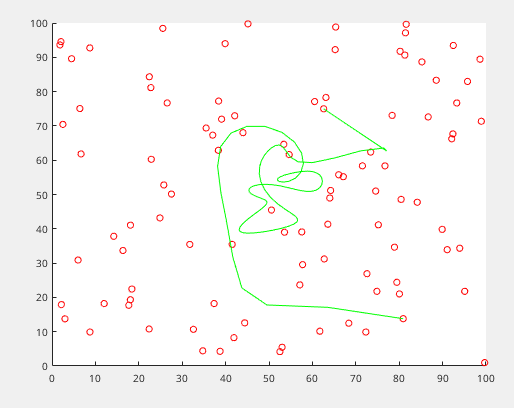
\includegraphics[width=0.8\linewidth]{figs/03-curve.png}
  \caption{Curve for test 3}
  \label{fig:03-curve}
\end{figure}

\begin{figure}
	\centering
	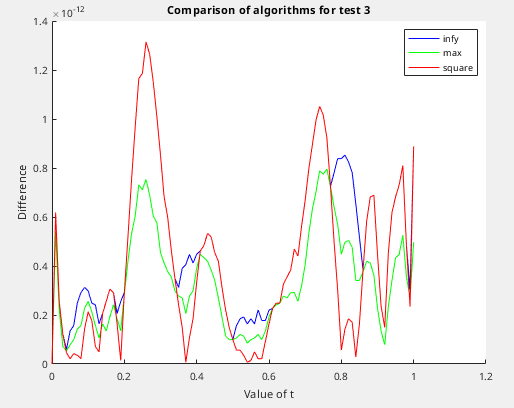
\includegraphics[width=0.8\linewidth]{figs/03-diffs.png}
	\caption{Comparison of algorithms for test 3}
	\label{fig:03-diffs}
\end{figure}

\begin{figure}
	\centering
	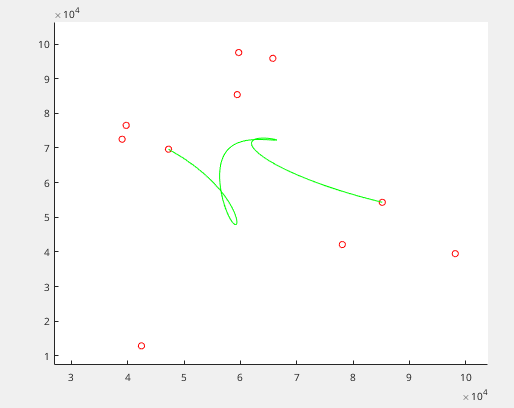
\includegraphics[width=0.8\linewidth]{figs/04-curve.png}
	\caption{Curve for test 4}
	\label{fig:04-curve}
\end{figure}

\begin{figure}
	\centering
	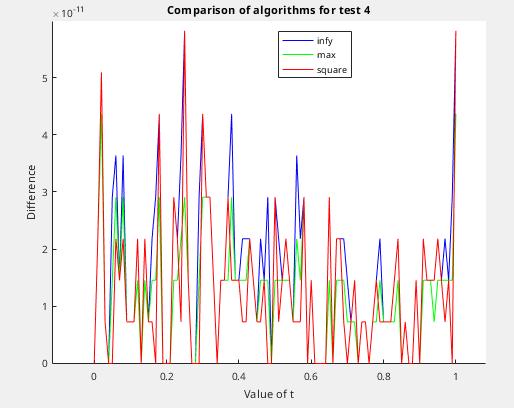
\includegraphics[width=0.8\linewidth]{figs/04-diffs.png}
	\caption{Comparison of algorithms for test 4}
	\label{fig:04-diffs}
\end{figure}

\end{document}

